\documentclass[12pt, a4paper]{report}
\usepackage[top=1.0in, bottom=1.0in, left=0.8in, right=0.8in]{geometry}
\usepackage{graphicx}
\usepackage{amsmath}
\usepackage{listings}
\usepackage{fancyvrb}

 	
\title{\textbf{EE2703 : Applied Programming Lab \\ Assignment 5 \\ Laplace Equation}} 
\author{Aditya Nanda Kishore\\ EE20B062} 

\date{\today} % Date for the report

	
\begin{document}
		
\maketitle
\section*{Abstract}
We wish to solve for the currents in a resistor. The currents depend on the shape of the resistor and we also want to know which part of the resistor is likely to get hottest.The aim of this assignment is to 
\begin{itemize}
	\item Understand and Solve the 2D Laplace equation thoroughly with the help of python.
	\item Solving for currents using potentials
	\item Understand vectorization of code.
\end{itemize}

\section*{Introduction}
A wire is soldered to the middle of a copper plate and its voltage is held at 1 Volt. One side of the plate is grounded, while the remaining are floating. The plate is 1 cm by 1 cm in size.We will divide the plate into a 25X25 grid and try to find the potential at every point using Laplace equation and given boundary conditions, thereby we will find the current from potential gradient. 

\section*{Laplace Equation and Potential Array}
Our plate has a 1V region and grounded region.We know that form Ohm's Law

\begin{equation}
  \vec{J} = \sigma\vec{F}
\end{equation}

and Electric field is the gradient of the potential
\begin{equation}
  \vec{E} = -\Delta\phi
\end{equation}

and charge continuity equation is given by 
\begin{figure}[!tbh]
   	\centering
   	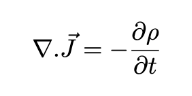
\includegraphics[scale=0.85]{A.png}
 \end{figure} 
 
 From those three equations, we get 
 \begin{figure}[!tbh]
   	\centering
   	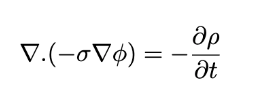
\includegraphics[scale=0.85]{B.png}
 \end{figure} 
 
 By rearranging terms and for DC currents, since gradient of $\rho$ with respect to time is zero, our equation becomes
  \begin{figure}[!tbh]
   	\centering
   	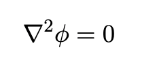
\includegraphics[scale=0.85]{D.png}
 \end{figure} 
   
This is the laplace equation. In 2D coordinates , It is 
  \begin{figure}[!tbh]
   	\centering
   	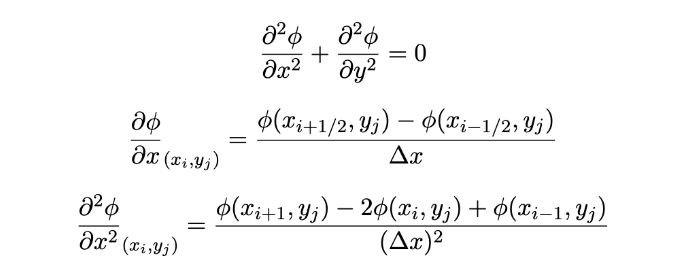
\includegraphics[scale=0.85]{E.png}
 \end{figure} 
\newpage
So we can conclude that, In our grid
  \begin{figure}[!tbh]
   	\centering
   	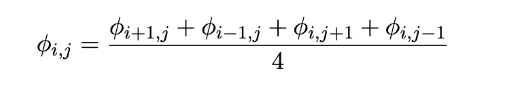
\includegraphics[scale=0.85]{F.png}
 \end{figure} 
   
\begin{itemize}
	\item So we define a potential array describing potential at every point, initially describing potential only at the wire part, where it's 1V. Now, from the equation above, the potential at any point should be the average of its neighbours.This approximation is taken to make the computation easier. We define error at every iteration as the maximum change in elements of $\phi$. Now we keep iterating till the error becomes very low
	\item Later for boundaries, we need to use boundary conditions from the electrodes. The top, left , right boundaries take the values of their immediate bottom, right, left row respectively whereas the bottom row is made zero as the bottom side is grounded.We are not considering any sudden change in potential as any gradient in potential in normal direction would mean current in normal direction. But since current is tangential at the edge of plate, Potential is almost constant at the edges of the plate.
\end{itemize}

Now, We import necessary modules and define $N_x = 25 $ and $N_y= 25 $ and $Niter = 1500$ Now the Potential array should have $N_y$ rows and $N_x$ columns. After defining that, since plate is 1 cm x 1 cm and is divided into $N_x$ units along x and $N_y$ units along y , we can define two \textit{linspace} arrays and later define meshgrids with the help of those 1D arrays

\begin{Verbatim}

from pylab import *
import mpl_toolkits.mplot3d.axes3d as p3
import matplotlib.pyplot as plt


Nx=25; # size along x
Ny=25; # size along y
radius=8;# radius of central lead
Niter=1500; # number of iterations to perform

phi = zeros((Ny,Nx))
y = linspace(-0.5, 0.5, num=Ny, dtype = float) 
x = linspace(-0.5, 0.5, num=Nx, dtype = float) 
Y,X= np.meshgrid(y,x)
\end{Verbatim}

To find the points which are inside the given radius, we have to use 
\begin{equation}
X^2 + Y^2 <= 0.35^2
\end{equation}
and later set the potential at all those points to 1V.Which can be implemented by 
\begin{Verbatim}
ii = np.where(X*X + Y*Y <= (0.35)**2 )
phi[ii] = 1
\end{Verbatim}

Plotting the Contour and Scatter plot of the Potential Array will give us this,
\begin{Verbatim}
plt.figure(0)
plt.scatter(x[ii[0]],y[ii[1]], c = 'red', label ="V = 1V")
plt.axis(xmin=-0.5, xmax=0.5, ymin=-0.5, ymax=0.5)
plt.title("Initial Potential Graph")
plt.legend(["V = 1V"])
plt.grid(True)
plt.show()

plt.contourf(x,y,phi)
plt.axis(xmin=-0.5, xmax=0.5, ymin=-0.5, ymax=0.5)
plt.title("Initial Potential Contour Plot")
plt.grid(True)
plt.show()
\end{Verbatim}

\begin{figure}[!tbh]
   	\centering
   	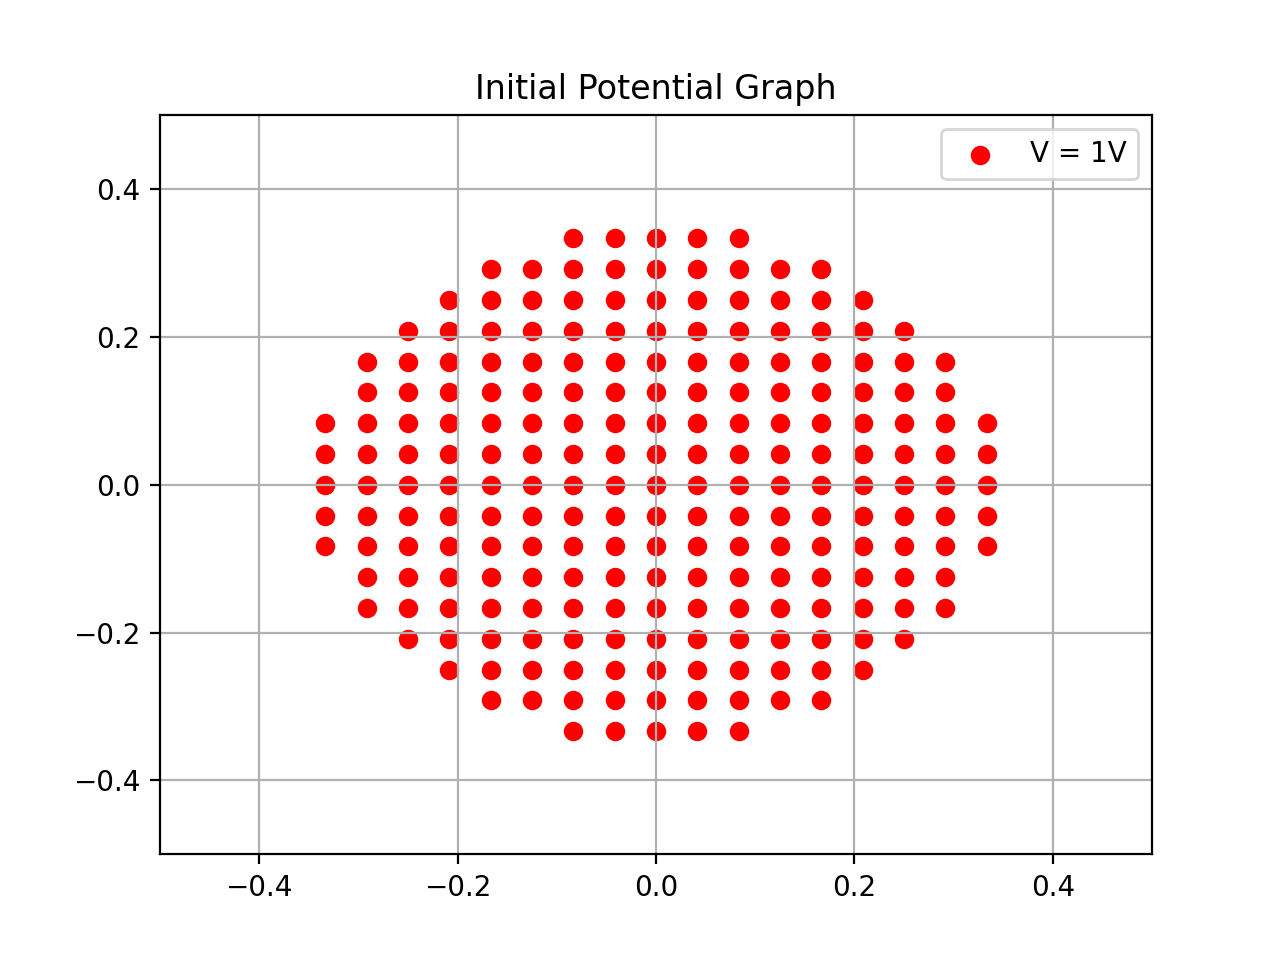
\includegraphics[scale=0.8]{Q1.png}
   	\caption{Initial Potential Scatter Plot}
 \end{figure} 


\begin{figure}[!tbh]
   	\centering
   	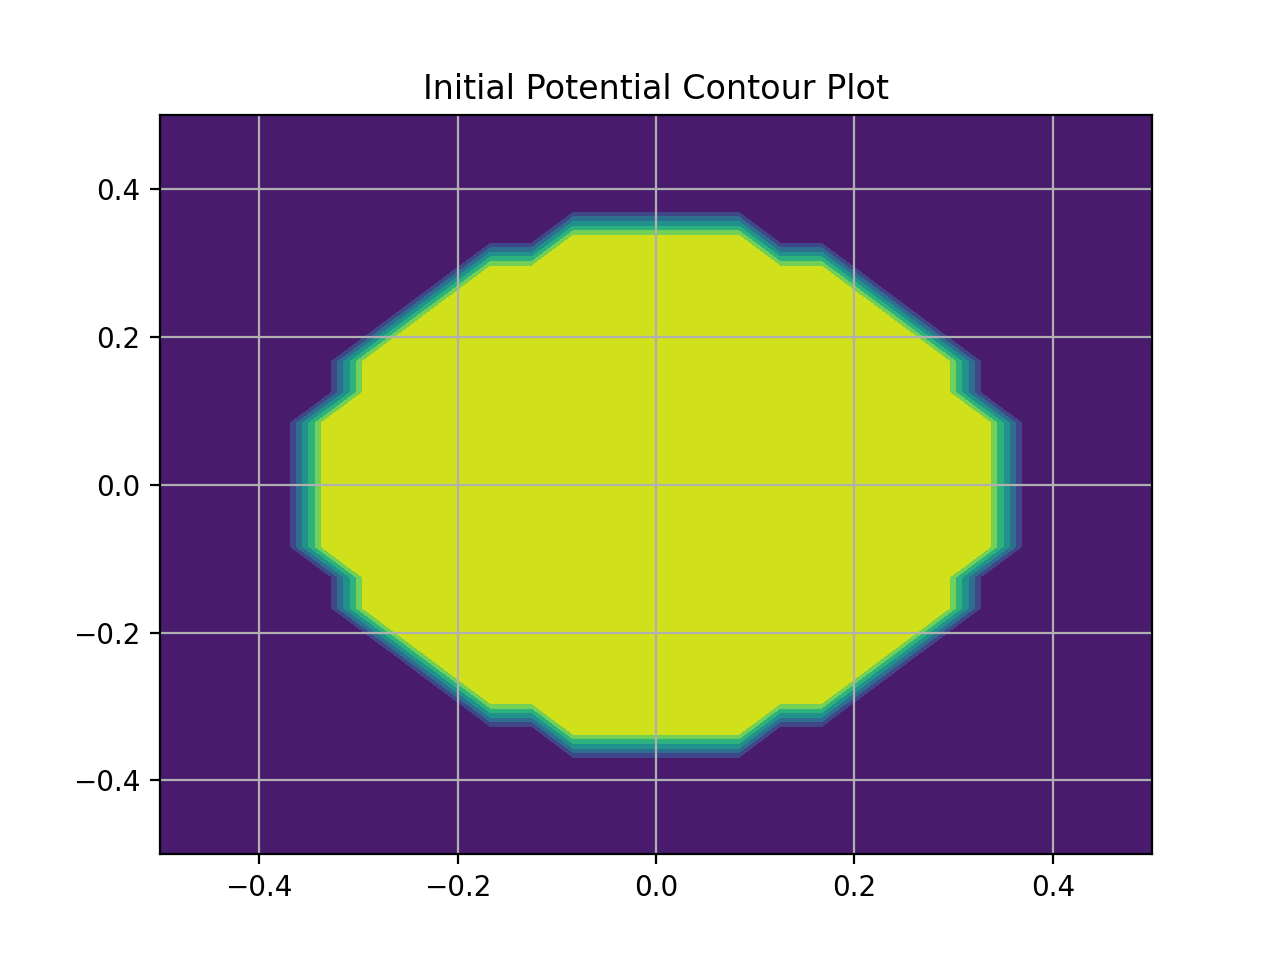
\includegraphics[scale=0.8]{Q1b.png}
   	\caption{Initial Potential Contour Plot}
   	\label{fig:allgraphs}
 \end{figure} 
 
 \section*{Potential Array Iteration}
 We have to update the potential according to the equation given below and vectorised code. We copy the $\phi$ and We calculate the $\phi[1:-1]$ part of the array using 4 sub arrays as shown below, which basically basically comprise the respectively directed matrix. For this I have defined a function and later for boundaries, I have defined another function for boundary that sets the boundary conditions.
 
  \begin{figure}[!tbh]
   	\centering
   	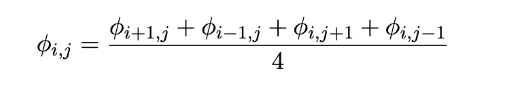
\includegraphics[scale=0.85]{F.png}
 \end{figure} 

\begin{Verbatim}
errors= []
n = np.arange(0, Niter)
def iterate(oldphi):
    phi = np.zeros(shape(oldphi))
    phi[1:-1,1:-1]=0.25*(oldphi[1:-1,0:-2] + oldphi[1:-1,2:] + oldphi[2:, 1:-1] + oldphi[0:-2, 1:-1])
    return phi

def set_boundaries(phi):
    phi[1:-1,0]=phi[1:-1,1]
    phi[1:-1,-1]=phi[1:-1,-2]
    phi[0, 0:] = phi[1, 0:]
    return phi
\end{Verbatim}
  
I have also defined an \textit{errors} list which I will be updating after every iteration in the coming code. So that I can analyse errors later.
\begin{Verbatim}

for i in range(Niter):
    oldphi=phi.copy()
    phi = iterate(oldphi)
    phi = set_boundaries(phi)
    phi[ii]=1.0
    errors.append((abs(phi-oldphi)).max())

errors = np.array(errors)
\end{Verbatim}

\section*{Errors}

Now, to analyse the error, I am plotting the error vs n in semi-log and log-log scale and also every 50th error.
\begin{Verbatim}
plt.semilogy(n, errors)
plt.title("Error vs Iterations Semi-log Plot ")
plt.show()

plt.loglog(n, errors)
plt.title("Error vs Iterations log-log Plot ")
plt.show()

plt.plot(n[::50] ,errors[::50])
plt.title("Every 50th Error-Individual Values")
plt.show()
\end{Verbatim}

\begin{figure}[!tbh]
   	\centering
   	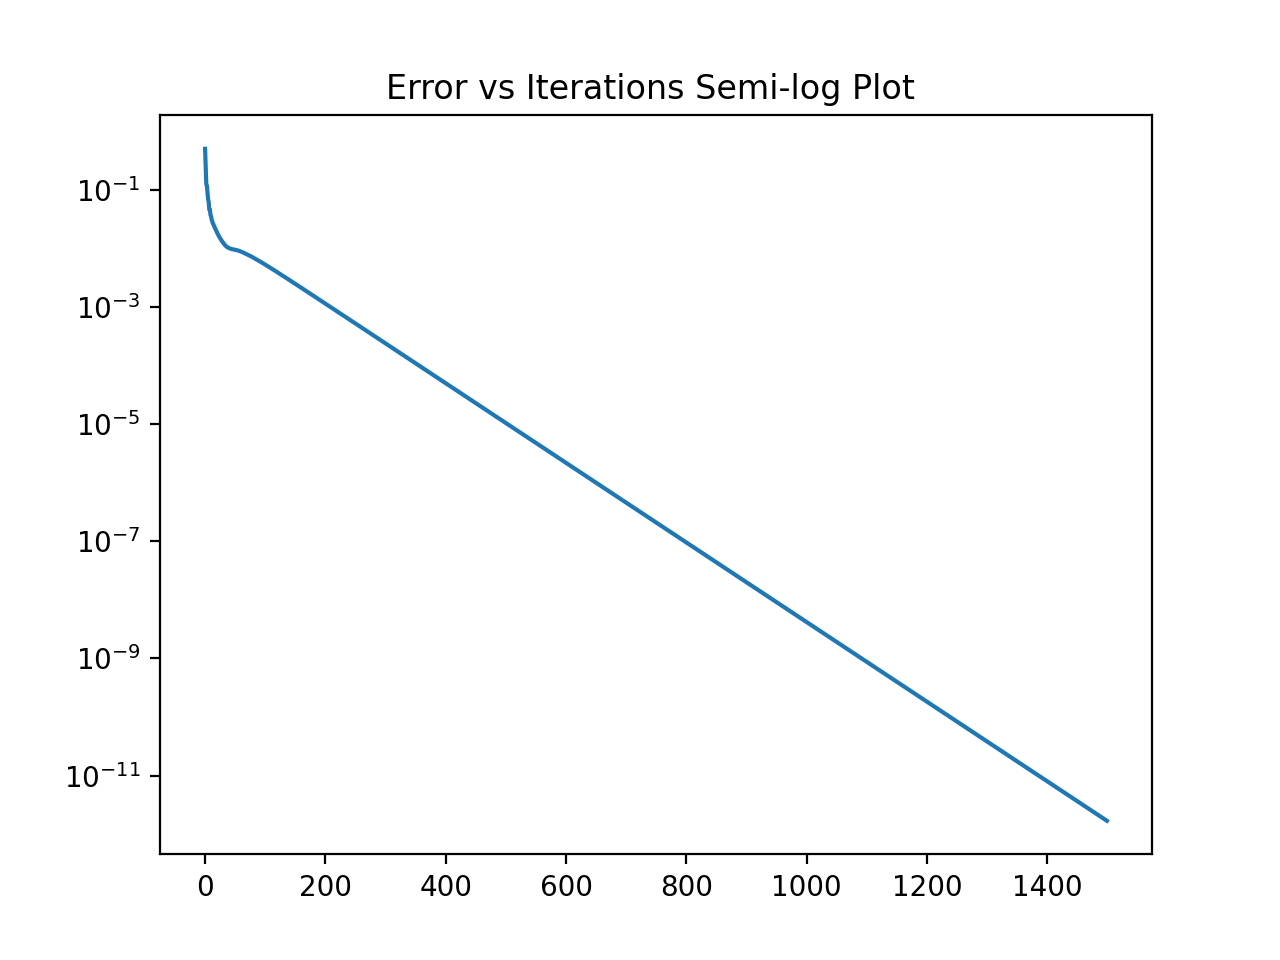
\includegraphics[scale=0.75]{Q2a.png}
   	\caption{Semi-log Error Plot}
   	\label{fig:allgraphs}
 \end{figure} 
 
 \begin{figure}[!tbh]
   	\centering
   	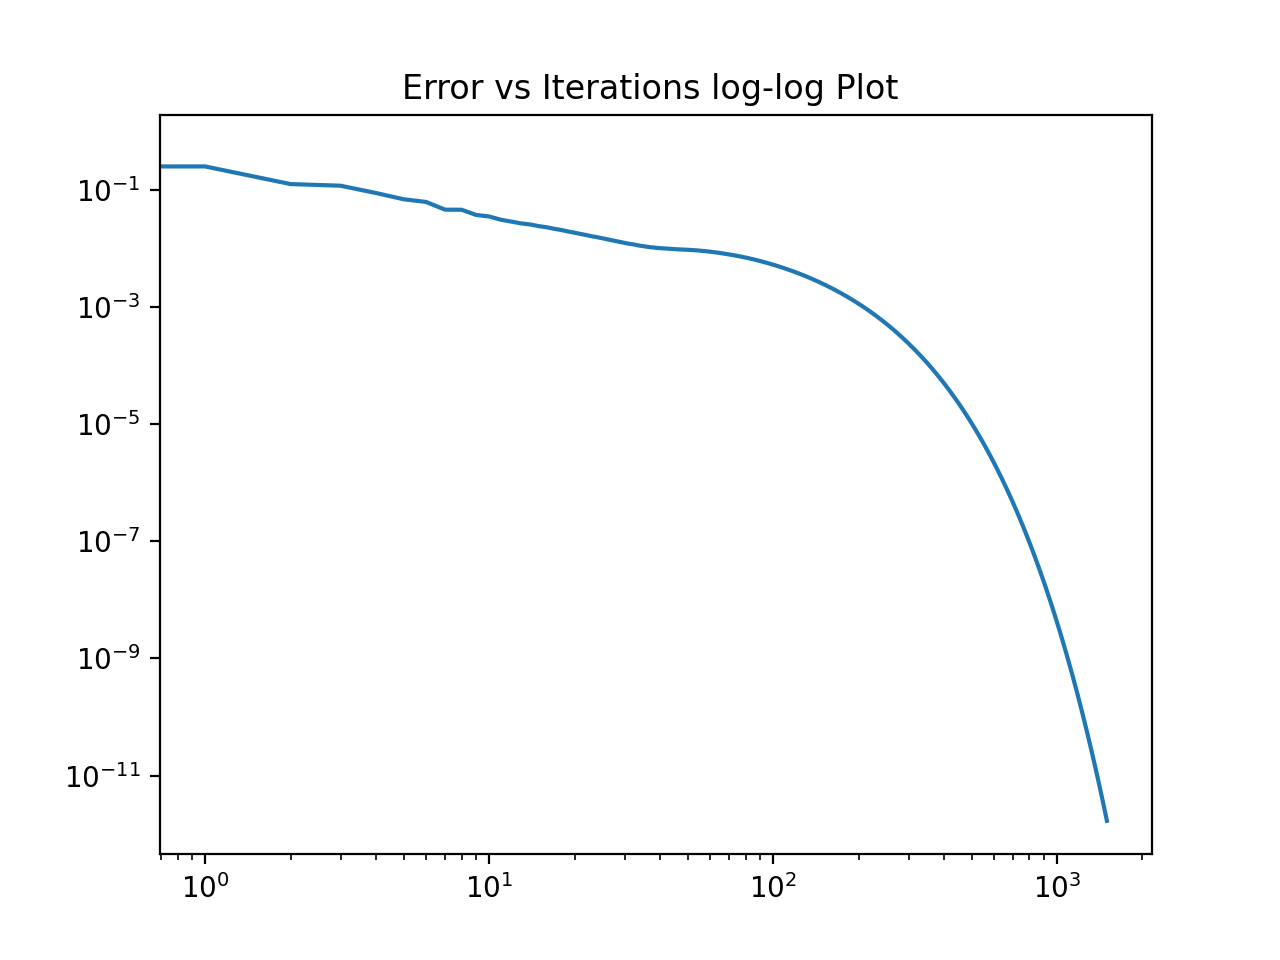
\includegraphics[scale=0.75]{Q2b.png}
   	\caption{Log-log Error Plot}
   	\label{fig:allgraphs}
 \end{figure} 
 \begin{figure}[!tbh]
   	\centering
   	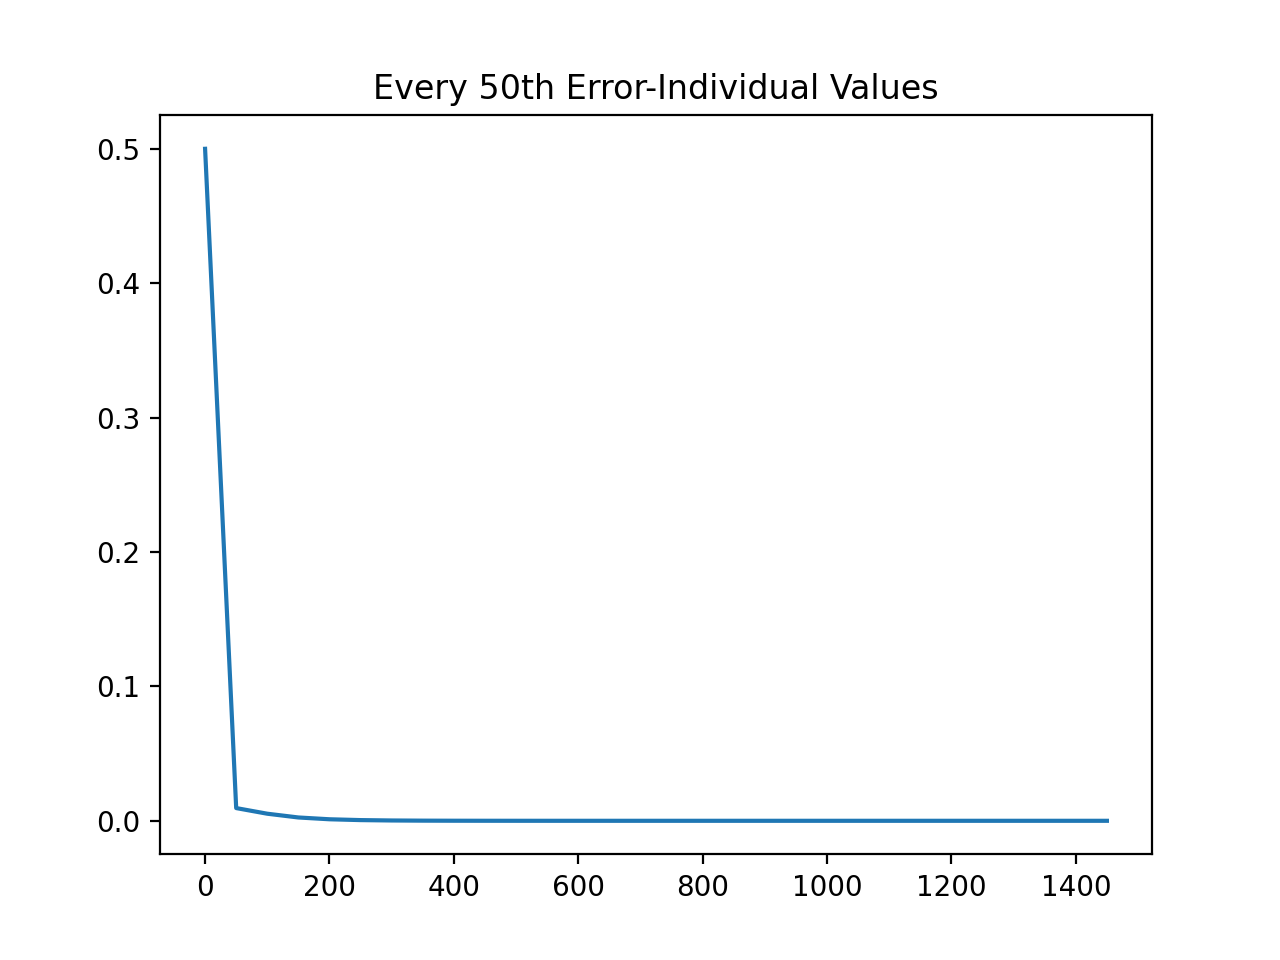
\includegraphics[scale=0.75]{Q2c.png}
   	\caption{Error Plot}
   	\label{fig:allgraphs}
 \end{figure} 
 
 We can see that log-log plot gives a reasonably straight line upto about 500 iterations, but beyond that, we get into the exponential regime. Now, the Semi-log plot is a straight line after 500 iterations. So we can take the fit to be of form
\begin{equation}
y = Ae^{Bn}
\end{equation}
\begin{equation}
logy = logA + Bn
\end{equation}
Hence, Graph is straight line in semi-log. Since we are trying to find the perfect fits, We have to find A,B using the data set here. We are going to use least squares method from the above equation, for this. We shall call them $A_0$ and $B_0$.We are going to change the dataset by considering the values after n = 500  and find new A,B.We shall call them $A_1$ and $B_1$
\begin{Verbatim}
M_0 = c_[np.ones(Niter), np.arange(Niter)]
c_all = np.linalg.lstsq(M_0,  np.log(errors), rcond=None)
a0, b0 = np.exp(c_all[0][0]), c_all[0][1]

M_1 = c_[np.ones(Niter-500), np.arange(500, Niter) ]
c_500 = np.linalg.lstsq(M_1, np.log(errors[500:]),rcond = None)
a1, b1 = np.exp(c_500[0][0]), c_500[0][1]
\end{Verbatim}

We get our final values as
\begin{itemize}
	\item $A_0 = 0.02621556381508562 $ and $B_0 = -0.015655263499125868$ 
	\item $A_1 = 0.02604396045065288 $ and $B_1 = -0.01564806811615406 $
\end{itemize}

By Drawing graphs from this , we get 
\begin{Verbatim}
# Plotting of the actual and expected error in semilog, for  all values
plt.semilogy(n, errors)
plt.semilogy(n, a0* np.exp(b0*n))
plt.legend(['Errors', 'Fit for all errors'])
plt.show()

# Plotting of the actual and expected error in semilog, for all values above n = 500
plt.semilogy(n[500:], errors[500:])
plt.semilogy(n[500:], a1* np.exp(b1*n[500:]),  linewidth = 3)
plt.legend(['Errors','Fit for values after 500'])
plt.show()
\end{Verbatim}

\begin{figure}[!tbh]
   	\centering
   	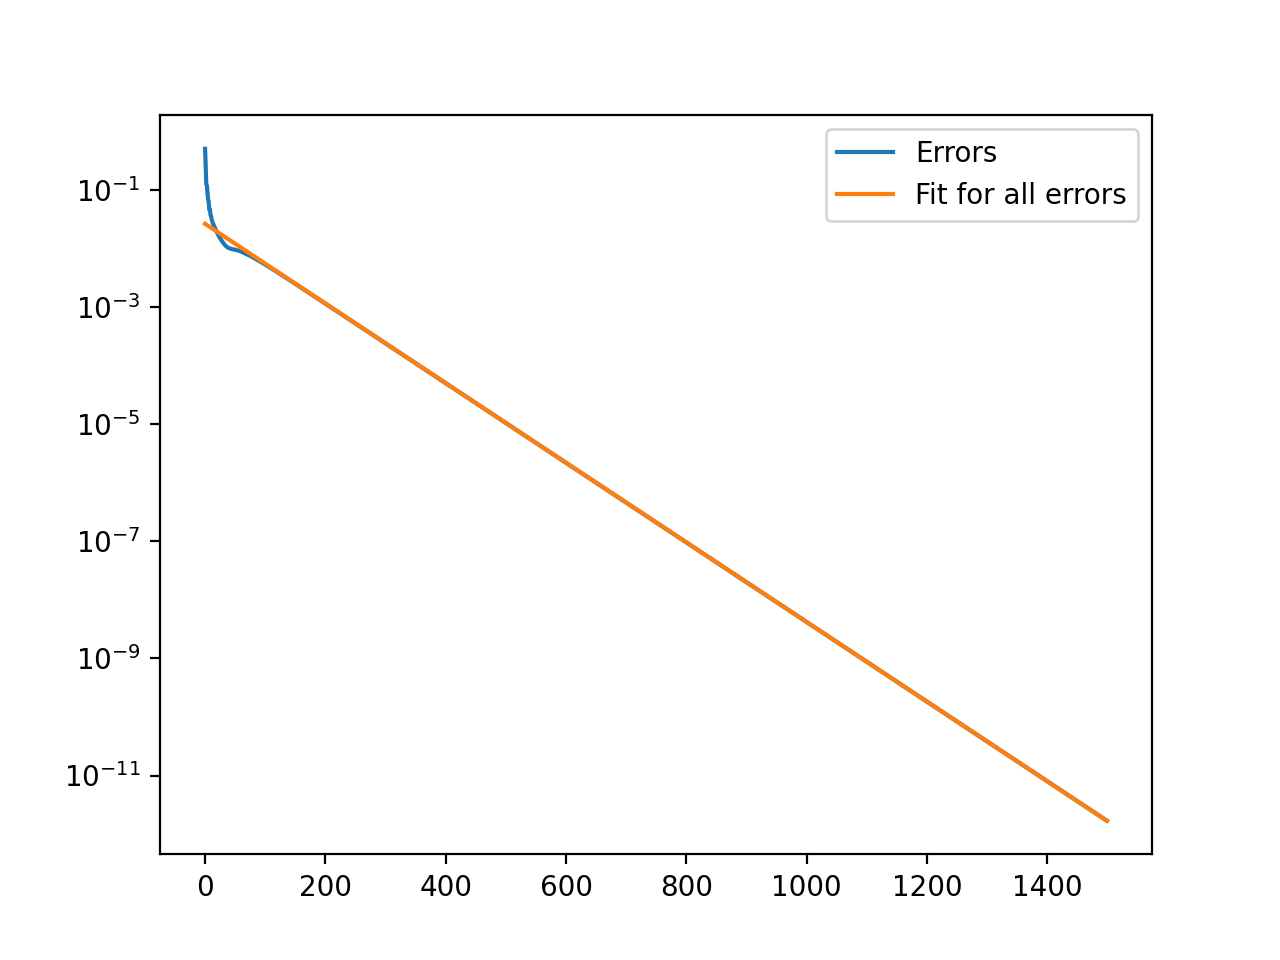
\includegraphics[scale=0.84]{Q3a.png}
	\caption{Error Plot and Fit 1}
   	\label{fig:allgraphs}
 \end{figure} 

\begin{figure}[!tbh]
   	\centering
   	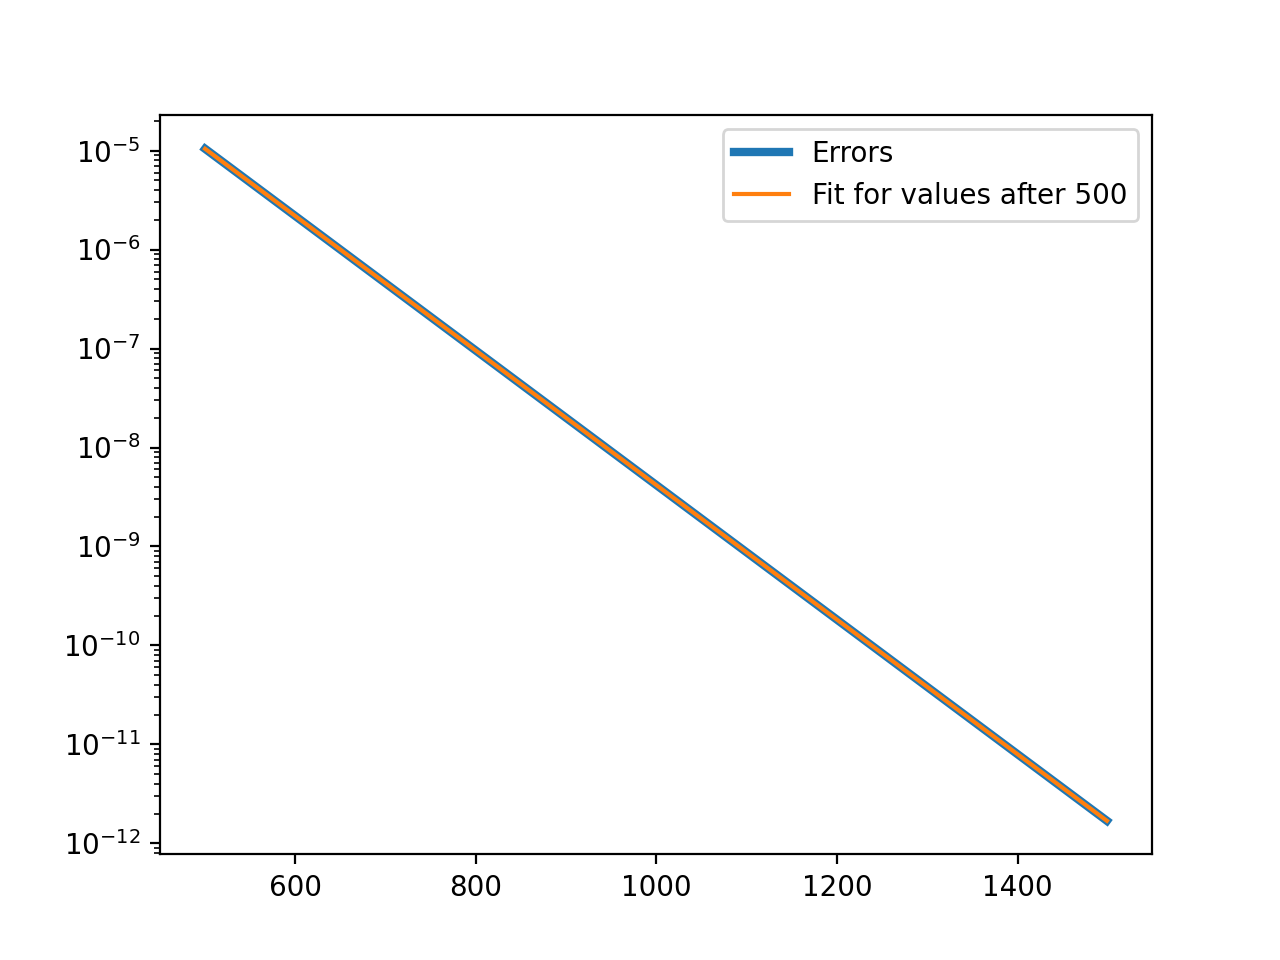
\includegraphics[scale=0.84]{Q3b.png}
   	\caption{Error Plot and Fit 2}
   	\label{fig:allgraphs}
 \end{figure} 
 
 \newpage
Clearly, Straight line is a really good approximation after n = 500, whereas the Error diverges a lot in the beginning i.e., for small n


\section*{Surface and Contour plot of Potential}
Since, We have a new potential array, we can plot the surface and contour plot of potential to get a more clear idea of how potential gradient is 
\begin{Verbatim}
# Plotting the surface plots of phi (potential).
fig1=plt.figure(4)     # open a new figure
ax=p3.Axes3D(fig1) # Axes3D is the means to do a surface plot
surf = ax.plot_surface(Y, X, phi.T, rstride=1, cstride=1, cmap=cm.jet)
plt.title('The 3-D surface plot of the potential')
plt.show()

# Plotting of the contour of phi (potential).
plt.contourf(-X, -Y, phi.T)
plt.scatter(x[ii[0]],y[ii[1]], c = 'red', label ="V = 1V")
plt.title("Contour plot of potential")
plt.colorbar()
plt.grid(True)
plt.show()
\end{Verbatim}


\begin{figure}[!tbh]
   	\centering
   	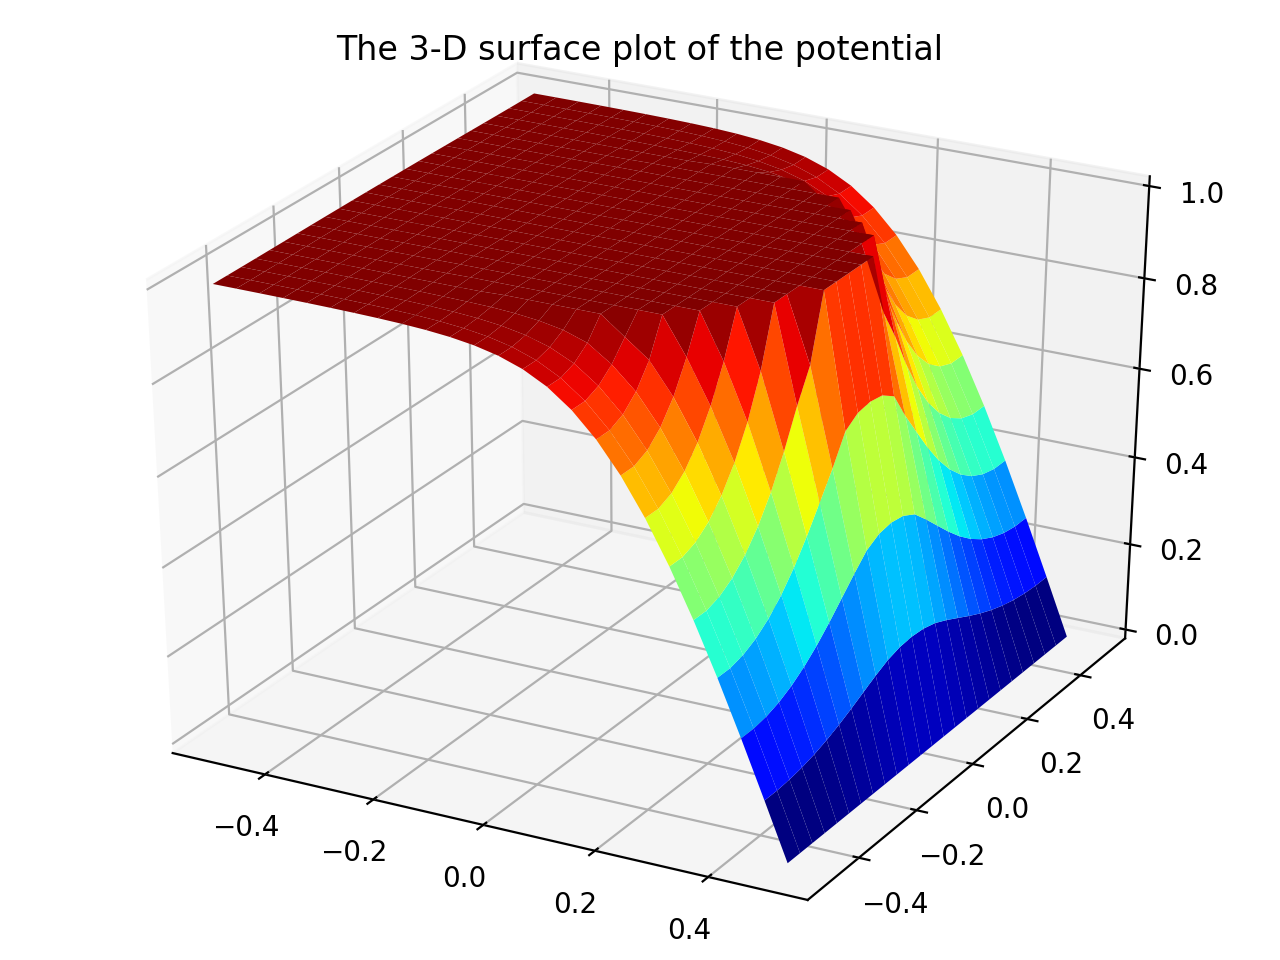
\includegraphics[scale=0.75]{Q4.png}
	\caption{Surface Plot}
   	\label{fig:allgraphs}
 \end{figure} 

\begin{figure}[!tbh]
   	\centering
   	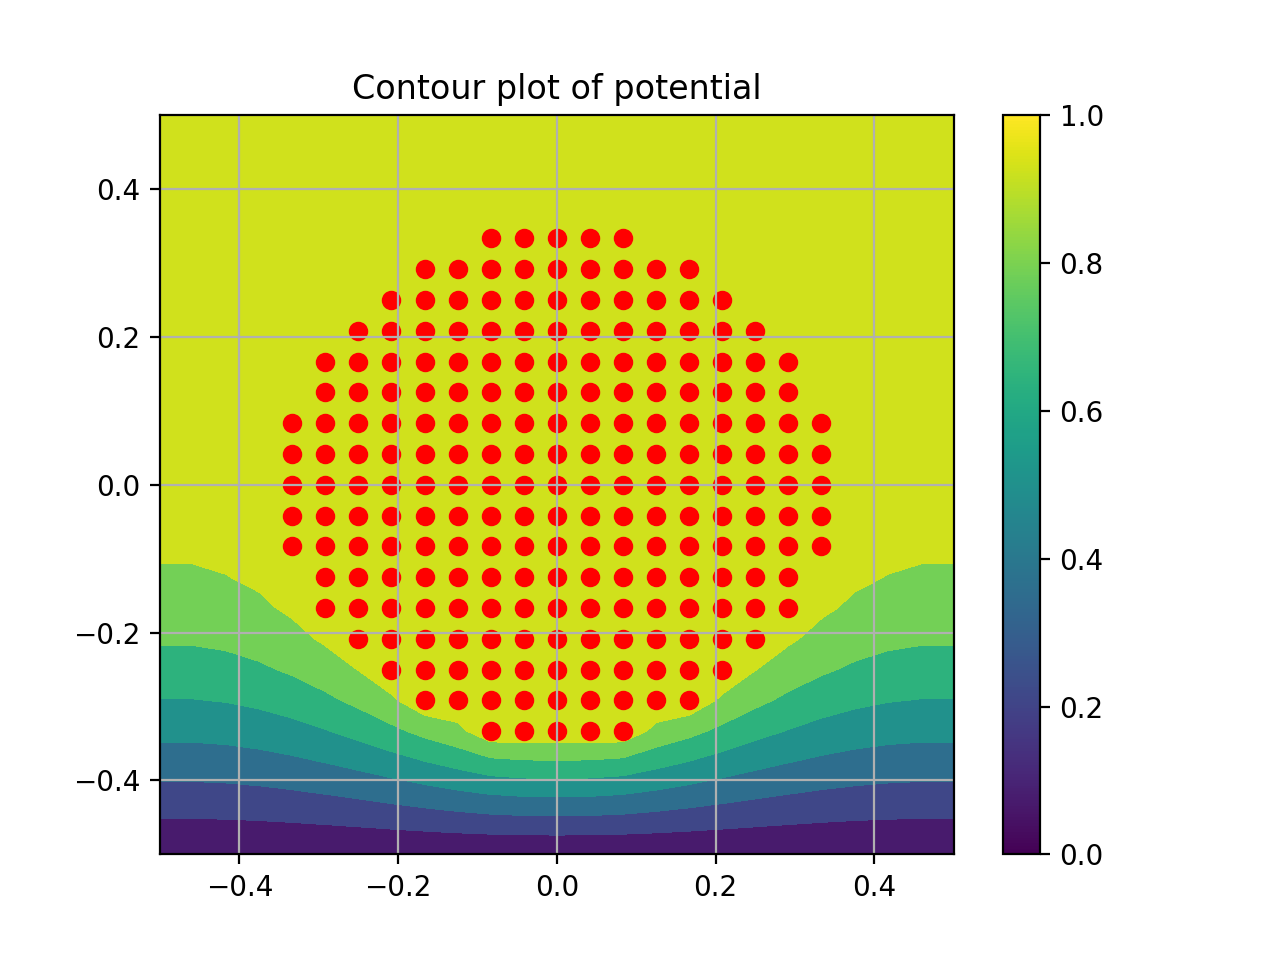
\includegraphics[scale=0.75]{Q5.png}
   	\caption{Contour Plot(Red dots represent potential at electrodes, they aren't a part of contour)}
   	\label{fig:allgraphs}
 \end{figure} 
 
 Clearly, Potential Gradient is much higher in the bottom part of the plate and there is very little to no potential gradient at the top of the plate  from the contour plot 
 
 \newpage
 \section*{Vector Plot of Currents}
 Since Electric field is negative of potential gradient , and $\vec{J}$ is directly proportional to $\vec{E}$, we get 
 \begin{equation}
 \vec{J} = \sigma\vec{E}
 \end{equation}
  \begin{equation}
  \vec{J} = -\sigma\vec{\nabla\phi}
  \end{equation}
  Since we are only interested in current's direction, we can set $\sigma$ to a constant value, say 1.
  So now, our equations in scalar form are
   \begin{equation}
 J_x = -\frac{\partial\phi}{\partial x}
 \end{equation}
  
 \begin{equation}
 J_y = -\frac{\partial\phi}{\partial y}
 \end{equation}
 
For Programming this , we can use 
\begin{figure}[!tbh]
   	\centering
   	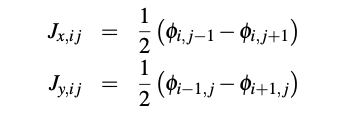
\includegraphics[scale=0.94]{G.png}
 \end{figure} 
We can use vectorized code again and plotting the vector plot would give us this,
\begin{Verbatim}
J_x = np.zeros((Ny, Nx))
J_y = np.zeros((Ny, Nx))
J_x[1:-1,1:-1] = 0.5*(-phi.T[1:-1,0:-2]+phi.T[1:-1,2:])
J_y[1:-1,1:-1] = 0.5*(phi.T[0:-2, 1:-1]-phi.T[2:, 1:-1])
plt.quiver(X,-Y,J_y,J_x, color='blue', scale = 5)
plt.scatter(x[ii[0]],y[ii[1]], c = 'red', linewidths = 0.5, label ="V = 1V")
plt.title("The vector plot of the current flow")
plt.show()

\end{Verbatim}

\begin{figure}[!tbh]
   	\centering
   	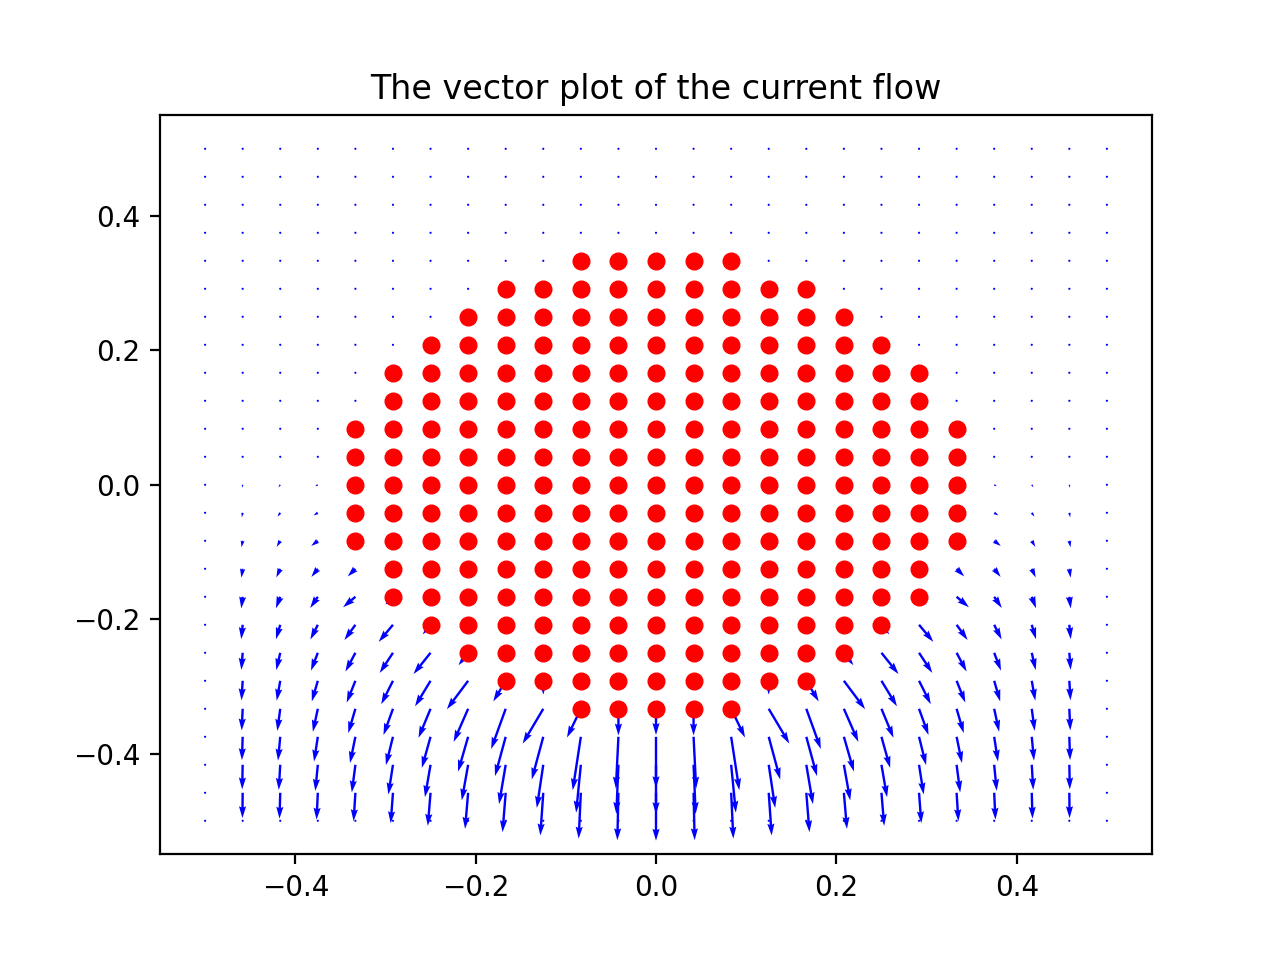
\includegraphics[scale=0.75]{Q6.png}
   	\caption{Current Plot}
   	\label{fig:allgraphs}
 \end{figure} 

As there is no potential gradient at the top of the plate , there is no current at all in the top part. whereas potential gradient is high at the bottom part resulting in high currents at the bottom part of the plate and we can also observe that current direction is perpendicular to the potential contour for verification.

\hfill \break
Now, we also know that heat generated is $\vec{J}.\vec{E}$ and both the quantities are high at bottom when compared to centre of the plate, so obviously temperature should be high at the bottom of the plate. It is also intuitive that temperature should be high there as current is headed and accumulated at the bottom.

\section*{Conclusion}
\begin{itemize}
	\item$N_x$, $N_y$ and $Niter$ affect the accuracy of the potential plot. More every variable is, More the accuracy of $\phi$ is 
	\item Potential gradient is much higher in the bottom part of the plate and there is very little to no potential gradient at the top of the plate.
	\item Current vectors start at the centre of the plate and travel perpendicular to the potential contour and at the bottom of the plate they are almost in Y direction, concluding that there is no gradient in $\phi$ along X at the bottom of the plate
	\item As there is no current at the top of the plate, the dot product $\vec{J}.\vec{E}$(ohmic loss) is almost zero and at the bottom of the plate it is high and the plate gets hotter
	\item Laplace equation can't be solved without necessary boundary conditions and if they are provided we can solve for $\phi$ at any point in the space using the same.
	\item Vectorization of code is a good method to iterate arrays instead of explicit looping, indexing. The code is finally easy to read and concise too.
	
\end{itemize}


\end{document}